\section{Inserção}

\begin{frame}[fragile]{Inserção em árvores red-black}

    \begin{itemize}
        \item A inserção em uma árvore \textit{red-black} consiste em duas etapas

        \item A primeira é a inserção de um nó vermelho, nos mesmos moldes da inserção em
            uma árvore binária de busca

        \item A segunda etapa consiste em corrigir possíveis violações às propriedades de 
            uma árvore \textit{red-black}

        \item Observe que as propriedade 1 e 3 sempre serão verdadeiras

        \item As demais propriedades podem ser violadas, a depender do local onde a 
            inserção foi realizada

        \item São quatro cenários possíveis
    \end{itemize}

\end{frame}

\begin{frame}[fragile]{Rotinas básicas de inserção}
    \inputsnippet{cpp}{69}{89}{rb.cpp}
\end{frame}

\begin{frame}[fragile]{Cenário A: inserção em árvore vazia}

    \begin{itemize}
        \item Neste caso, a inserção é trivial, mas a propriedade 2 é violada

        \item A correção consiste em pintar a raiz com a cor preta

        \item Este processo adicionará uma unidade ao tamanho de todos os caminhos que 
            partem da raiz às folhas

        \item Assim, a propriedade 5 ficará preservada

        \item Segue abaixo uma visualização da inserção da informação 40 em uma árvore vazia:
    \end{itemize}

    \begin{figure}
    \centering
    
\begin{tikzpicture}
        \begin{scope}{shift={(3,0)}}
            \node[opacity=0] (X) at (-1, 2) { $1$ };
            \node[circle,draw,fill=red] (A) at (2, 2) { \textcolor{white}{40} };
            \node[circle,fill=black] (B) at (6, 2) { \textcolor{white}{40} };

            \draw[->] (3, 2) -- (5, 2);
            \draw[->] (-1, 2) -- (1, 2);
        \end{scope}
    \end{tikzpicture}
    \end{figure}

\end{frame}

\begin{frame}[fragile]{Restauração das propriedades no cenário A}
    \inputsnippet{cpp}{90}{94}{rb.cpp}
\end{frame}

\begin{frame}[fragile]{Cenário B: o pai do nó inserido é preto}

    \begin{itemize}
        \item Como o pai do nó inserido $n$ é preto, não há violação da propriedade 4

        \item Além disso, como $n$ é vermelho, o caminho da raiz até um de seus filhos mantém o
            mesmo número de nós pretos que haviam até a posição onde $n$ foi inserido

        \item Deste modo, não há violação da propriedade 5

        \item Como $n$ tem um pai preto, ele não é a raiz (pois a raiz não tem pai)

        \item Assim, não há violação da propriedade 2

        \item De fato, neste cenário não há necessidade de nenhuma correção após a inserção
    \end{itemize}

\end{frame}

\begin{frame}[fragile]{Exemplo de inserções no cenário B}

    \begin{tikzpicture}
        \begin{scope}{shift={(3,0)}}
            \node[opacity=0] (X) at (-1, 2) { $1$ };
            \node[anchor=west] at (0, 8) { Informação a ser inserida: \textcolor{blue}{17} };
            \node[circle,fill=black] (B) at (4, 6) { \textcolor{white}{40} };
        \end{scope}
    \end{tikzpicture}

\end{frame}

\begin{frame}[fragile]{Exemplo de inserções no cenário B}

    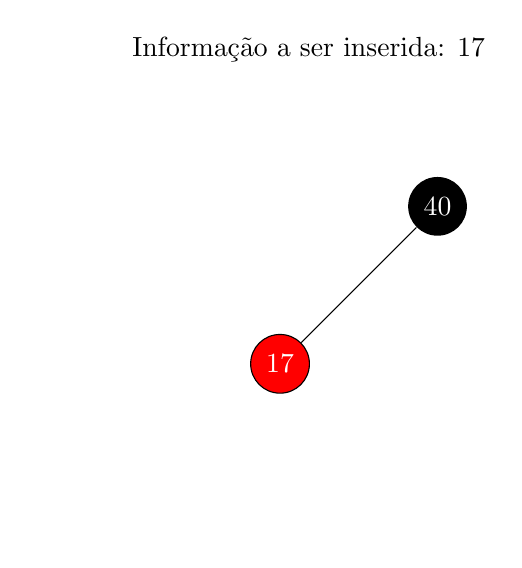
\begin{tikzpicture}
        \begin{scope}{shift={(3,0)}}
            \node[opacity=0] (X) at (-1, 2) { $1$ };
            \node[anchor=west] at (0, 8) { Informação a ser inserida: \textcolor{black}{17} };
            \node[circle,fill=black] (A) at (4, 6) { \textcolor{white}{40} };
            \node[circle,draw,fill=red] (B) at (2, 4) { \textcolor{white}{17} };

            \draw (A) -- (B);
        \end{scope}
    \end{tikzpicture}

\end{frame}

\begin{frame}[fragile]{Exemplo de inserções no cenário B}

    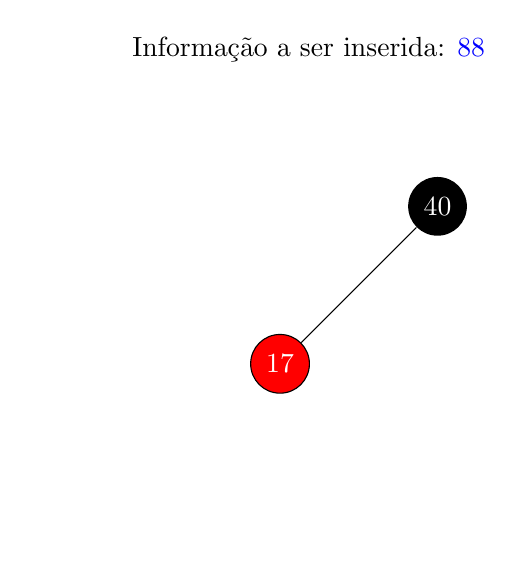
\begin{tikzpicture}
        \begin{scope}{shift={(3,0)}}
            \node[opacity=0] (X) at (-1, 2) { $1$ };
            \node[anchor=west] at (0, 8) { Informação a ser inserida: \textcolor{blue}{88} };
            \node[circle,fill=black] (A) at (4, 6) { \textcolor{white}{40} };
            \node[circle,draw,fill=red] (B) at (2, 4) { \textcolor{white}{17} };

            \draw (A) -- (B);
        \end{scope}
    \end{tikzpicture}

\end{frame}

\begin{frame}[fragile]{Exemplo de inserções no cenário B}

    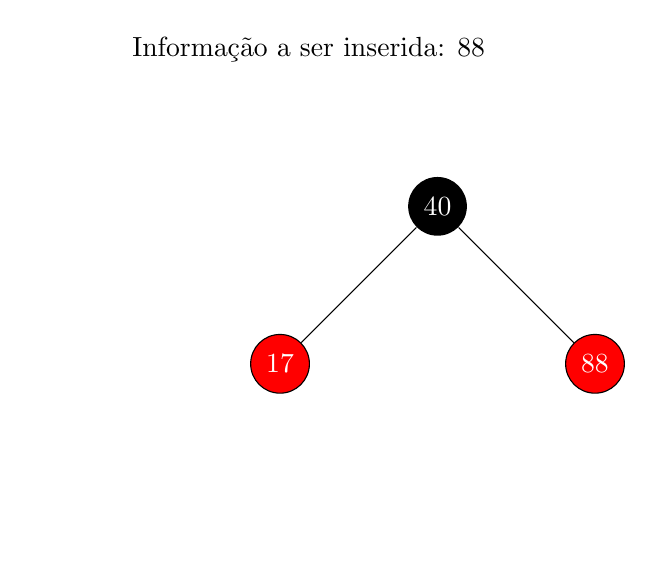
\begin{tikzpicture}
        \begin{scope}{shift={(3,0)}}
            \node[opacity=0] (X) at (-1, 2) { $1$ };
            \node[anchor=west] at (0, 8) { Informação a ser inserida: \textcolor{black}{88} };
            \node[circle,fill=black] (A) at (4, 6) { \textcolor{white}{40} };
            \node[circle,draw,fill=red] (B) at (2, 4) { \textcolor{white}{17} };
            \node[circle,draw,fill=red] (C) at (6, 4) { \textcolor{white}{88} };

            \draw (A) -- (B);
            \draw (A) -- (C);
        \end{scope}
    \end{tikzpicture}

\end{frame}

\begin{frame}[fragile]{Cenário C: o pai e o tio do nó inserido são vermelhos}

    \begin{itemize}
        \item Neste cenário, o pai e o tio do nó inserido $n$ são ambos vermelhos

        \item Como $n$ também é vermelho, há uma violação da propriedade 4

        \item Se o avô se tornar vermelho, e o pai e o tio se tornarem pretos, a violação da
            propriedade 4 é corrigida

        \item Esta mudança também não viola a propriedade 5, pois o número de nós pretos
            nos caminhos muda

        \item Contudo, se o avô for a raiz, a propriedade 2 passa a ser violada

        \item Caso contrário, pode existir uma violação da propriedade 4, se o bisavô for
            vermelho

        \item Para evitar tais violações, é preciso reiniciar a rotina de correção no avô
    \end{itemize}

\end{frame}

\begin{frame}[fragile]{Exemplo de inserções no cenário C}

    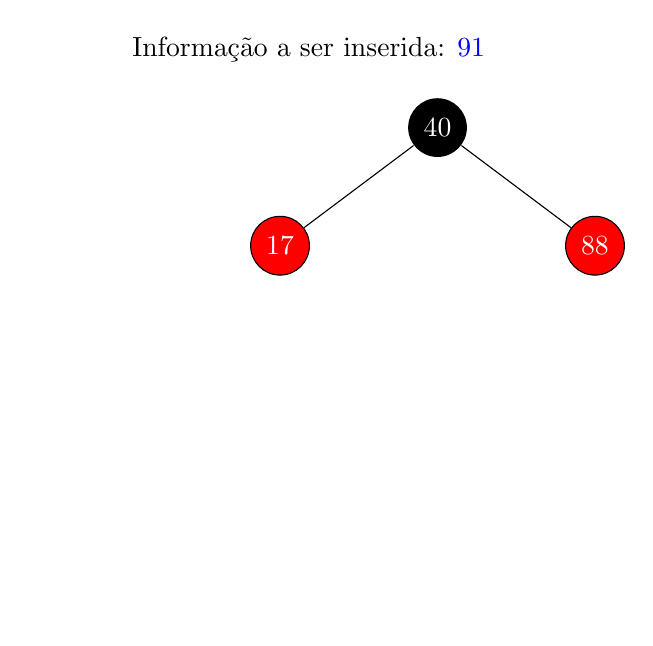
\begin{tikzpicture}
        \begin{scope}{shift={(3,0)}}
            \node[opacity=0] (X) at (-1, 1) { $1$ };
            \node[anchor=west] at (0, 8) { Informação a ser inserida: \textcolor{blue}{91} };
            \node[circle,fill=black] (A) at (4, 7) { \textcolor{white}{40} };
            \node[circle,draw,fill=red] (B) at (2, 5.5) { \textcolor{white}{17} };
            \node[circle,draw,fill=red] (C) at (6, 5.5) { \textcolor{white}{88} };

            \draw (A) -- (B);
            \draw (A) -- (C);
        \end{scope}
    \end{tikzpicture}

\end{frame}

\begin{frame}[fragile]{Exemplo de inserções no cenário C}

    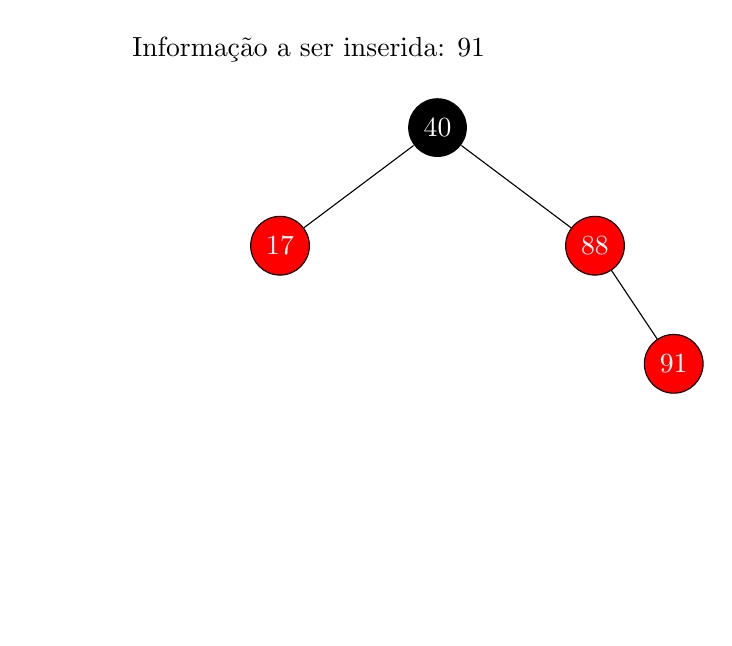
\begin{tikzpicture}
        \begin{scope}{shift={(3,0)}}
            \node[opacity=0] (X) at (-1, 1) { $1$ };
            \node[anchor=west] at (0, 8) { Informação a ser inserida: \textcolor{black}{91} };
            \node[circle,fill=black] (A) at (4, 7) { \textcolor{white}{40} };
            \node[circle,draw,fill=red] (B) at (2, 5.5) { \textcolor{white}{17} };
            \node[circle,draw,fill=red] (C) at (6, 5.5) { \textcolor{white}{88} };
            \node[circle,draw,fill=red] (D) at (7, 4) { \textcolor{white}{91} };

            \draw (A) -- (B);
            \draw (A) -- (C);
            \draw (C) -- (D);
        \end{scope}
    \end{tikzpicture}

\end{frame}

\begin{frame}[fragile]{Exemplo de inserções no cenário C}

    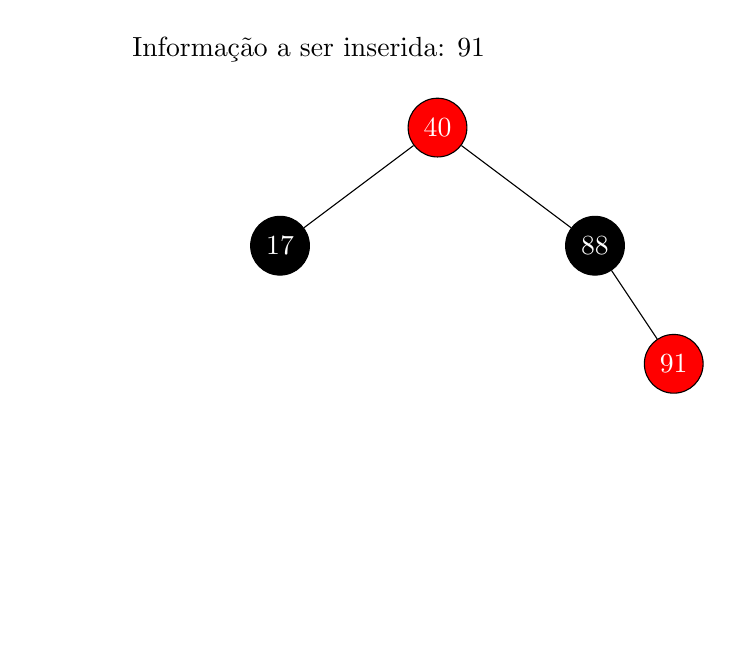
\begin{tikzpicture}
        \begin{scope}{shift={(3,0)}}
            \node[opacity=0] (X) at (-1, 1) { $1$ };
            \node[anchor=west] at (0, 8) { Informação a ser inserida: \textcolor{black}{91} };
            \node[circle,draw,fill=red] (A) at (4, 7) { \textcolor{white}{40} };
            \node[circle,draw,fill=black] (B) at (2, 5.5) { \textcolor{white}{17} };
            \node[circle,draw,fill=black] (C) at (6, 5.5) { \textcolor{white}{88} };
            \node[circle,draw,fill=red] (D) at (7, 4) { \textcolor{white}{91} };

            \draw (A) -- (B);
            \draw (A) -- (C);
            \draw (C) -- (D);
        \end{scope}
    \end{tikzpicture}

\end{frame}

\begin{frame}[fragile]{Exemplo de inserções no cenário C}

    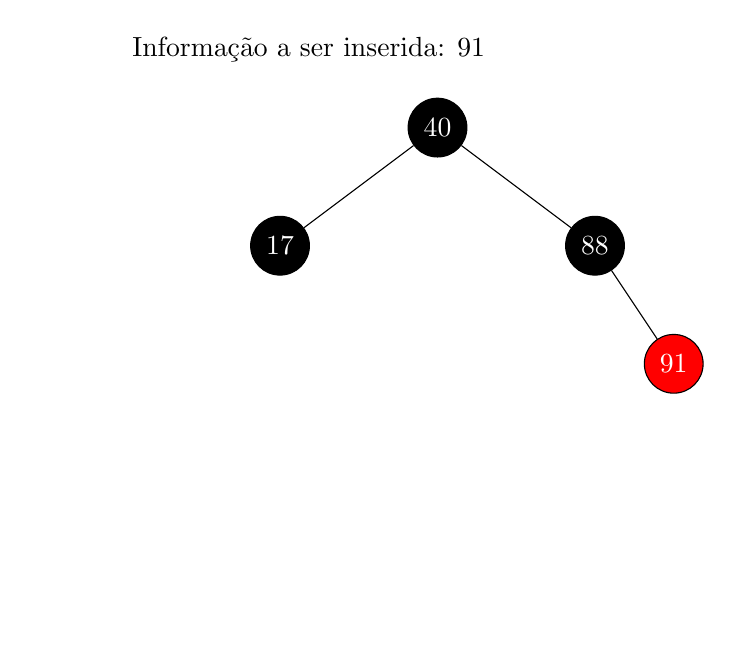
\begin{tikzpicture}
        \begin{scope}{shift={(3,0)}}
            \node[opacity=0] (X) at (-1, 1) { $1$ };
            \node[anchor=west] at (0, 8) { Informação a ser inserida: \textcolor{black}{91} };
            \node[circle,draw,fill=black] (A) at (4, 7) { \textcolor{white}{40} };
            \node[circle,draw,fill=black] (B) at (2, 5.5) { \textcolor{white}{17} };
            \node[circle,draw,fill=black] (C) at (6, 5.5) { \textcolor{white}{88} };
            \node[circle,draw,fill=red] (D) at (7, 4) { \textcolor{white}{91} };

            \draw (A) -- (B);
            \draw (A) -- (C);
            \draw (C) -- (D);
        \end{scope}
    \end{tikzpicture}

\end{frame}

\begin{frame}[fragile]{Restauração das propriedades nos cenários B e C}
    \inputsnippet{cpp}{95}{105}{rb.cpp}
\end{frame}

\begin{frame}[fragile]{Cenário D: pai vermelho, tio preto}

    \begin{itemize}
        \item Neste último cenário, é necessário utilizar rotações de modo a reposicionar
            o pai na posição do avô

        \item A direção da rotação é definida de acordo com a posição do pai em relação ao 
            avô: se for o filho à esquerda, a rotação é para a direita, e vice-versa

        \item Também é necessária a troca de cores entre o pai e o avô após a rotação

        \item Esta troca restaura as violação à propriedade 4 e não viola a propriedade 5

        \item Há, porém, um caso especial: se o filho tiver em direção oposta a que o pai ocupa
            em relação ao avô

       \item Neste caso, é necessária uma rotação para colocar o filho na posição do pai

       \item Deste modo, ambos passaram a ter a mesma direção em relação ao avô
    \end{itemize}

\end{frame}

\begin{frame}[fragile]{Exemplo de inserções no cenário D}

    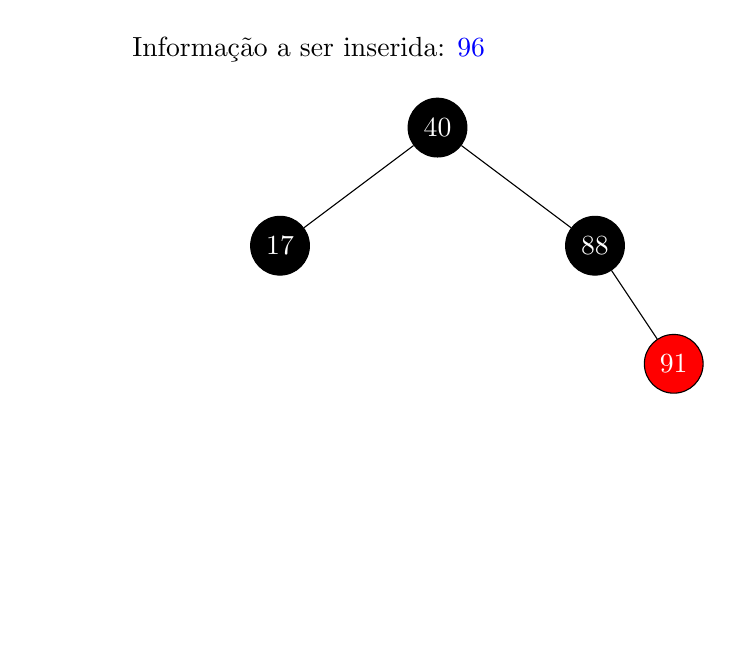
\begin{tikzpicture}
        \begin{scope}{shift={(3,0)}}
            \node[opacity=0] (X) at (-1, 1) { $1$ };
            \node[anchor=west] at (0, 8) { Informação a ser inserida: \textcolor{blue}{96} };
            \node[circle,draw,fill=black] (A) at (4, 7) { \textcolor{white}{40} };
            \node[circle,draw,fill=black] (B) at (2, 5.5) { \textcolor{white}{17} };
            \node[circle,draw,fill=black] (C) at (6, 5.5) { \textcolor{white}{88} };
            \node[circle,draw,fill=red] (D) at (7, 4) { \textcolor{white}{91} };

            \draw (A) -- (B);
            \draw (A) -- (C);
            \draw (C) -- (D);
        \end{scope}
    \end{tikzpicture}

\end{frame}

\begin{frame}[fragile]{Exemplo de inserções no cenário D}

    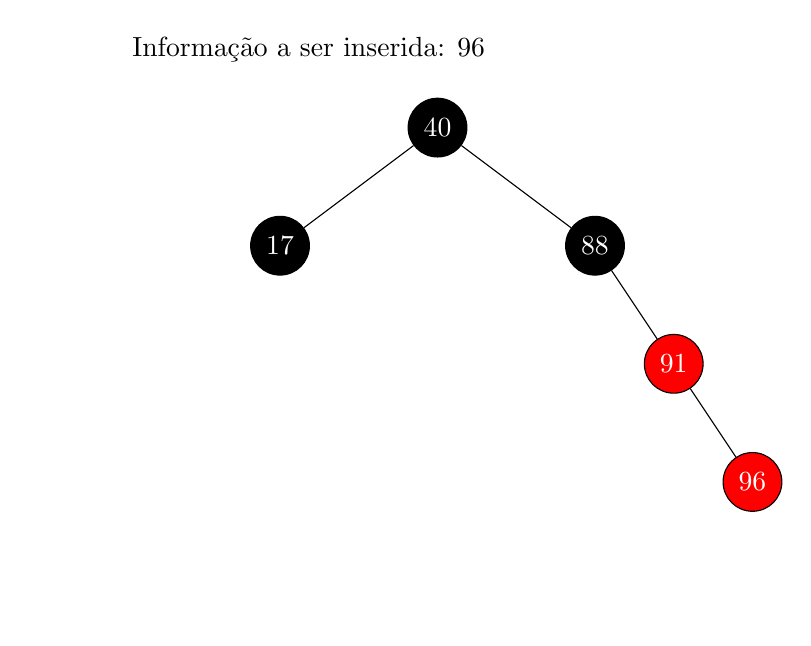
\begin{tikzpicture}
        \begin{scope}{shift={(3,0)}}
            \node[opacity=0] (X) at (-1, 1) { $1$ };
            \node[anchor=west] at (0, 8) { Informação a ser inserida: \textcolor{black}{96} };
            \node[circle,draw,fill=black] (A) at (4, 7) { \textcolor{white}{40} };
            \node[circle,draw,fill=black] (B) at (2, 5.5) { \textcolor{white}{17} };
            \node[circle,draw,fill=black] (C) at (6, 5.5) { \textcolor{white}{88} };
            \node[circle,draw,fill=red] (D) at (7, 4) { \textcolor{white}{91} };
            \node[circle,draw,fill=red] (E) at (8, 2.5) { \textcolor{white}{96} };

            \draw (A) -- (B);
            \draw (A) -- (C);
            \draw (C) -- (D);
            \draw (D) -- (E);
        \end{scope}
    \end{tikzpicture}

\end{frame}

\begin{frame}[fragile]{Exemplo de inserções no cenário D}

    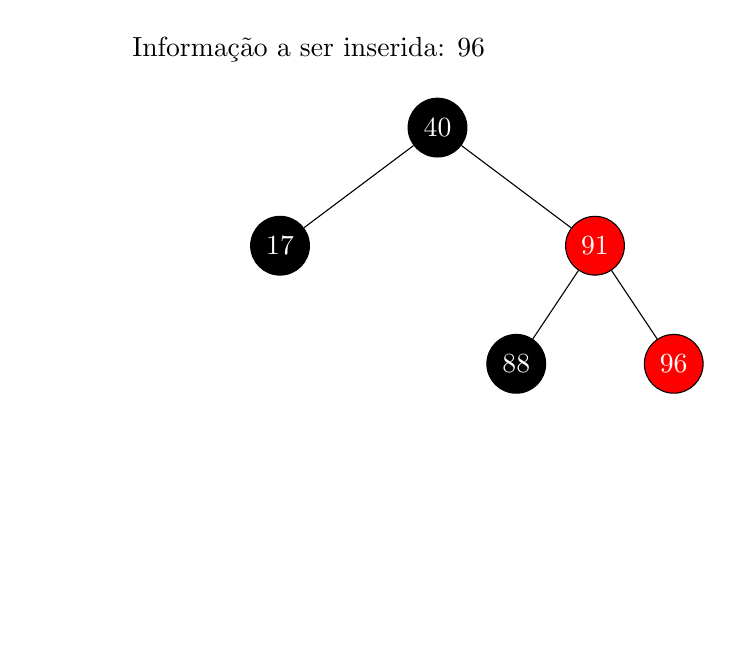
\begin{tikzpicture}
        \begin{scope}{shift={(3,0)}}
            \node[opacity=0] (X) at (-1, 1) { $1$ };
            \node[anchor=west] at (0, 8) { Informação a ser inserida: \textcolor{black}{96} };
            \node[circle,draw,fill=black] (A) at (4, 7) { \textcolor{white}{40} };
            \node[circle,draw,fill=black] (B) at (2, 5.5) { \textcolor{white}{17} };
            \node[circle,draw,fill=black] (C) at (5, 4) { \textcolor{white}{88} };
            \node[circle,draw,fill=red] (D) at (6, 5.5) { \textcolor{white}{91} };
            \node[circle,draw,fill=red] (E) at (7, 4) { \textcolor{white}{96} };

            \draw (A) -- (B);
            \draw (A) -- (D);
            \draw (C) -- (D);
            \draw (D) -- (E);
        \end{scope}
    \end{tikzpicture}

\end{frame}

\begin{frame}[fragile]{Exemplo de inserções no cenário D}

    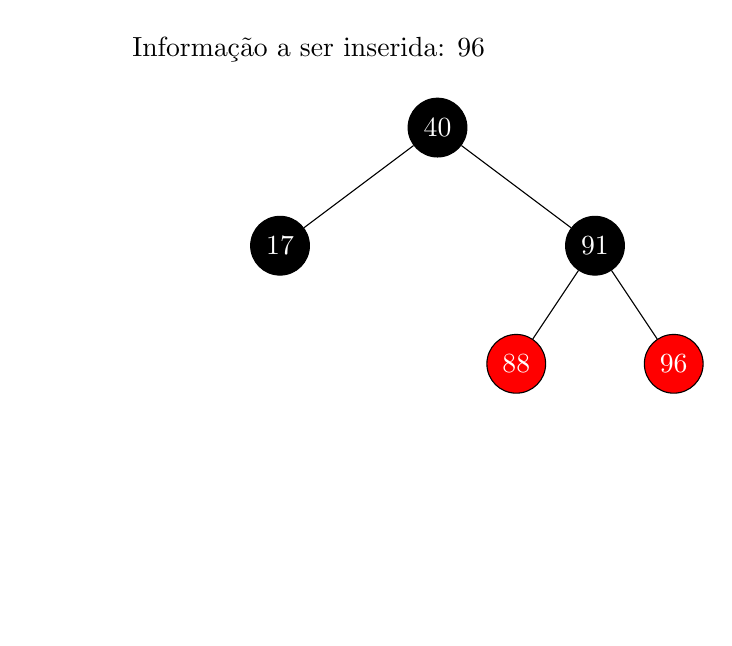
\begin{tikzpicture}
        \begin{scope}{shift={(3,0)}}
            \node[opacity=0] (X) at (-1, 1) { $1$ };
            \node[anchor=west] at (0, 8) { Informação a ser inserida: \textcolor{black}{96} };
            \node[circle,draw,fill=black] (A) at (4, 7) { \textcolor{white}{40} };
            \node[circle,draw,fill=black] (B) at (2, 5.5) { \textcolor{white}{17} };
            \node[circle,draw,fill=red] (C) at (5, 4) { \textcolor{white}{88} };
            \node[circle,draw,fill=black] (D) at (6, 5.5) { \textcolor{white}{91} };
            \node[circle,draw,fill=red] (E) at (7, 4) { \textcolor{white}{96} };

            \draw (A) -- (B);
            \draw (A) -- (D);
            \draw (C) -- (D);
            \draw (D) -- (E);
        \end{scope}
    \end{tikzpicture}

\end{frame}

\begin{frame}[fragile]{Exemplo de inserções no cenário D}

    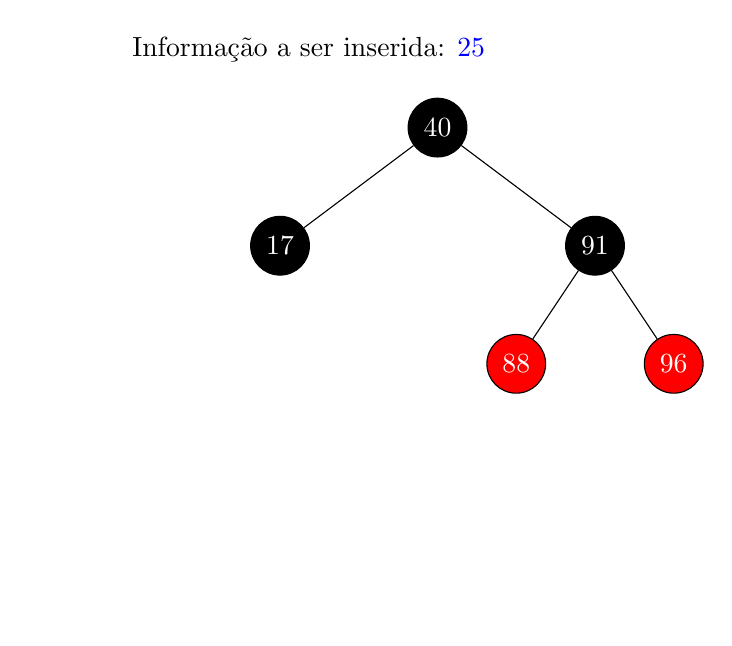
\begin{tikzpicture}
        \begin{scope}{shift={(3,0)}}
            \node[opacity=0] (X) at (-1, 1) { $1$ };
            \node[anchor=west] at (0, 8) { Informação a ser inserida: \textcolor{blue}{25} };
            \node[circle,draw,fill=black] (A) at (4, 7) { \textcolor{white}{40} };
            \node[circle,draw,fill=black] (B) at (2, 5.5) { \textcolor{white}{17} };
            \node[circle,draw,fill=red] (C) at (5, 4) { \textcolor{white}{88} };
            \node[circle,draw,fill=black] (D) at (6, 5.5) { \textcolor{white}{91} };
            \node[circle,draw,fill=red] (E) at (7, 4) { \textcolor{white}{96} };

            \draw (A) -- (B);
            \draw (A) -- (D);
            \draw (C) -- (D);
            \draw (D) -- (E);
        \end{scope}
    \end{tikzpicture}

\end{frame}

\begin{frame}[fragile]{Exemplo de inserções no cenário D}

    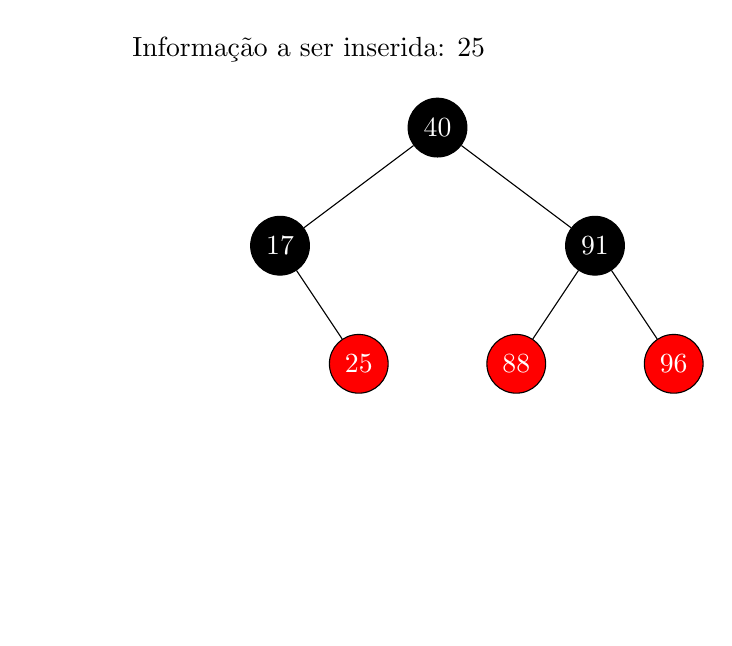
\begin{tikzpicture}
        \begin{scope}{shift={(3,0)}}
            \node[opacity=0] (X) at (-1, 1) { $1$ };
            \node[anchor=west] at (0, 8) { Informação a ser inserida: \textcolor{black}{25} };
            \node[circle,draw,fill=black] (A) at (4, 7) { \textcolor{white}{40} };
            \node[circle,draw,fill=black] (B) at (2, 5.5) { \textcolor{white}{17} };
            \node[circle,draw,fill=red] (C) at (5, 4) { \textcolor{white}{88} };
            \node[circle,draw,fill=black] (D) at (6, 5.5) { \textcolor{white}{91} };
            \node[circle,draw,fill=red] (E) at (7, 4) { \textcolor{white}{96} };
            \node[circle,draw,fill=red] (F) at (3, 4) { \textcolor{white}{25} };

            \draw (A) -- (B);
            \draw (A) -- (D);
            \draw (C) -- (D);
            \draw (D) -- (E);
            \draw (B) -- (F);
        \end{scope}
    \end{tikzpicture}

\end{frame}

\begin{frame}[fragile]{Exemplo de inserções no cenário D}

    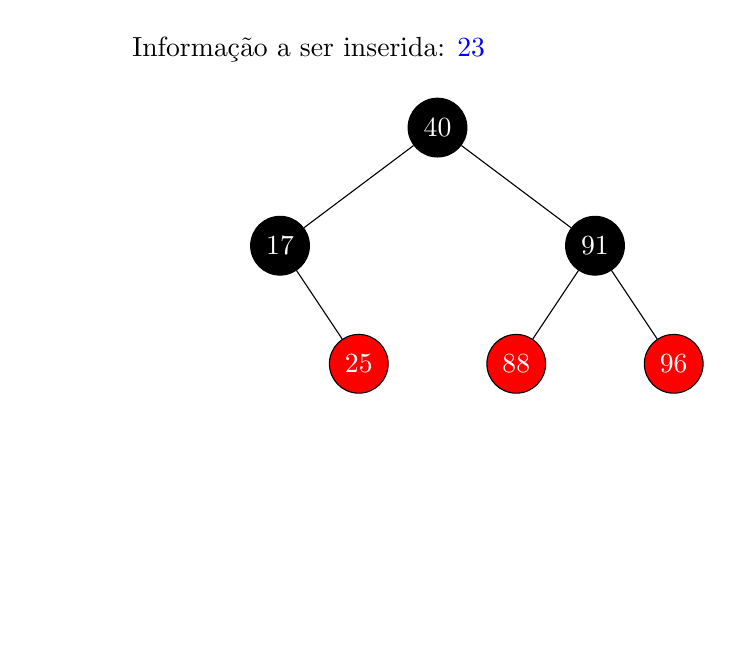
\begin{tikzpicture}
        \begin{scope}{shift={(3,0)}}
            \node[opacity=0] (X) at (-1, 1) { $1$ };
            \node[anchor=west] at (0, 8) { Informação a ser inserida: \textcolor{blue}{23} };
            \node[circle,draw,fill=black] (A) at (4, 7) { \textcolor{white}{40} };
            \node[circle,draw,fill=black] (B) at (2, 5.5) { \textcolor{white}{17} };
            \node[circle,draw,fill=red] (C) at (5, 4) { \textcolor{white}{88} };
            \node[circle,draw,fill=black] (D) at (6, 5.5) { \textcolor{white}{91} };
            \node[circle,draw,fill=red] (E) at (7, 4) { \textcolor{white}{96} };
            \node[circle,draw,fill=red] (F) at (3, 4) { \textcolor{white}{25} };

            \draw (A) -- (B);
            \draw (A) -- (D);
            \draw (C) -- (D);
            \draw (D) -- (E);
            \draw (B) -- (F);
        \end{scope}
    \end{tikzpicture}

\end{frame}

\begin{frame}[fragile]{Exemplo de inserções no cenário D}

    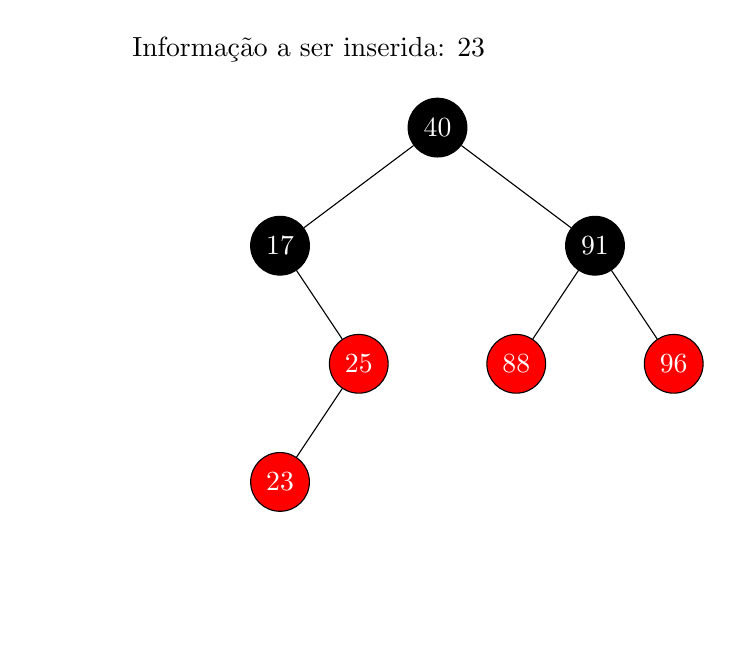
\begin{tikzpicture}
        \begin{scope}{shift={(3,0)}}
            \node[opacity=0] (X) at (-1, 1) { $1$ };
            \node[anchor=west] at (0, 8) { Informação a ser inserida: \textcolor{black}{23} };
            \node[circle,draw,fill=black] (A) at (4, 7) { \textcolor{white}{40} };
            \node[circle,draw,fill=black] (B) at (2, 5.5) { \textcolor{white}{17} };
            \node[circle,draw,fill=red] (C) at (5, 4) { \textcolor{white}{88} };
            \node[circle,draw,fill=black] (D) at (6, 5.5) { \textcolor{white}{91} };
            \node[circle,draw,fill=red] (E) at (7, 4) { \textcolor{white}{96} };
            \node[circle,draw,fill=red] (F) at (3, 4) { \textcolor{white}{25} };
            \node[circle,draw,fill=red] (G) at (2, 2.5) { \textcolor{white}{23} };

            \draw (A) -- (B);
            \draw (A) -- (D);
            \draw (C) -- (D);
            \draw (D) -- (E);
            \draw (B) -- (F);
            \draw (G) -- (F);
        \end{scope}
    \end{tikzpicture}

\end{frame}

\begin{frame}[fragile]{Exemplo de inserções no cenário D}

    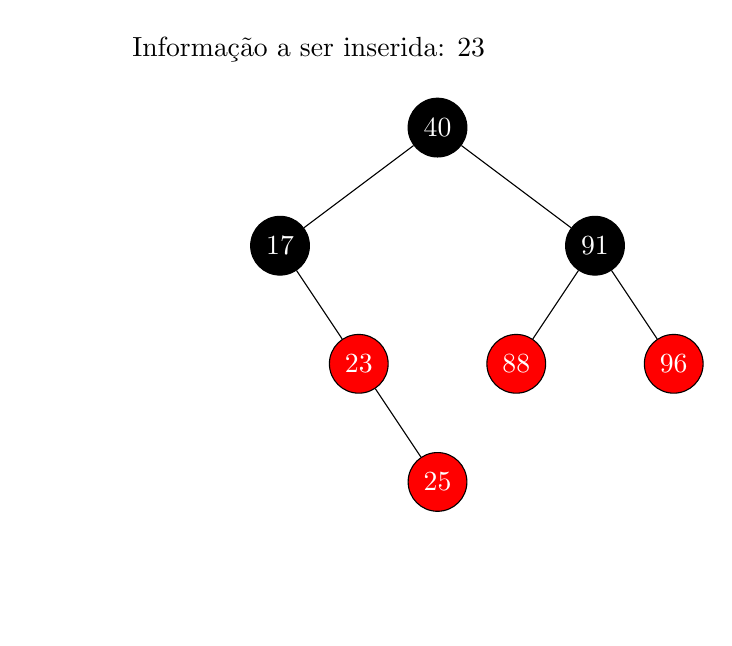
\begin{tikzpicture}
        \begin{scope}{shift={(3,0)}}
            \node[opacity=0] (X) at (-1, 1) { $1$ };
            \node[anchor=west] at (0, 8) { Informação a ser inserida: \textcolor{black}{23} };
            \node[circle,draw,fill=black] (A) at (4, 7) { \textcolor{white}{40} };
            \node[circle,draw,fill=black] (B) at (2, 5.5) { \textcolor{white}{17} };
            \node[circle,draw,fill=red] (C) at (5, 4) { \textcolor{white}{88} };
            \node[circle,draw,fill=black] (D) at (6, 5.5) { \textcolor{white}{91} };
            \node[circle,draw,fill=red] (E) at (7, 4) { \textcolor{white}{96} };
            \node[circle,draw,fill=red] (F) at (3, 4) { \textcolor{white}{23} };
            \node[circle,draw,fill=red] (G) at (4, 2.5) { \textcolor{white}{25} };

            \draw (A) -- (B);
            \draw (A) -- (D);
            \draw (C) -- (D);
            \draw (D) -- (E);
            \draw (B) -- (F);
            \draw (G) -- (F);
        \end{scope}
    \end{tikzpicture}

\end{frame}

\begin{frame}[fragile]{Exemplo de inserções no cenário D}

    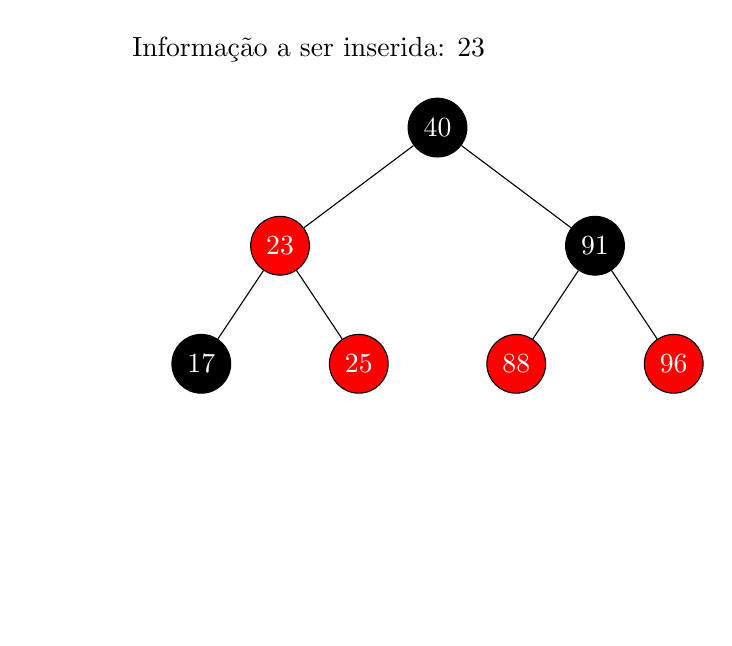
\begin{tikzpicture}
        \begin{scope}{shift={(3,0)}}
            \node[opacity=0] (X) at (-1, 1) { $1$ };
            \node[anchor=west] at (0, 8) { Informação a ser inserida: \textcolor{black}{23} };
            \node[circle,draw,fill=black] (A) at (4, 7) { \textcolor{white}{40} };
            \node[circle,draw,fill=black] (B) at (1, 4) { \textcolor{white}{17} };
            \node[circle,draw,fill=red] (C) at (5, 4) { \textcolor{white}{88} };
            \node[circle,draw,fill=black] (D) at (6, 5.5) { \textcolor{white}{91} };
            \node[circle,draw,fill=red] (E) at (7, 4) { \textcolor{white}{96} };
            \node[circle,draw,fill=red] (F) at (2, 5.5) { \textcolor{white}{23} };
            \node[circle,draw,fill=red] (G) at (3, 4) { \textcolor{white}{25} };

            \draw (A) -- (F);
            \draw (A) -- (D);
            \draw (C) -- (D);
            \draw (D) -- (E);
            \draw (B) -- (F);
            \draw (G) -- (F);
        \end{scope}
    \end{tikzpicture}

\end{frame}

\begin{frame}[fragile]{Exemplo de inserções no cenário D}

    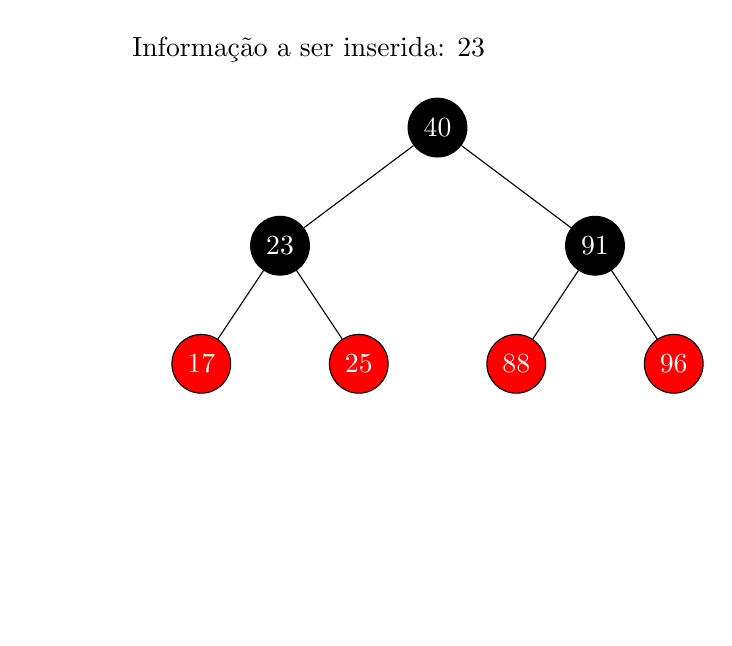
\begin{tikzpicture}
        \begin{scope}{shift={(3,0)}}
            \node[opacity=0] (X) at (-1, 1) { $1$ };
            \node[anchor=west] at (0, 8) { Informação a ser inserida: \textcolor{black}{23} };
            \node[circle,draw,fill=black] (A) at (4, 7) { \textcolor{white}{40} };
            \node[circle,draw,fill=red] (B) at (1, 4) { \textcolor{white}{17} };
            \node[circle,draw,fill=red] (C) at (5, 4) { \textcolor{white}{88} };
            \node[circle,draw,fill=black] (D) at (6, 5.5) { \textcolor{white}{91} };
            \node[circle,draw,fill=red] (E) at (7, 4) { \textcolor{white}{96} };
            \node[circle,draw,fill=black] (F) at (2, 5.5) { \textcolor{white}{23} };
            \node[circle,draw,fill=red] (G) at (3, 4) { \textcolor{white}{25} };

            \draw (A) -- (F);
            \draw (A) -- (D);
            \draw (C) -- (D);
            \draw (D) -- (E);
            \draw (B) -- (F);
            \draw (G) -- (F);
        \end{scope}
    \end{tikzpicture}

\end{frame}

\begin{frame}[fragile]{Restauração das propriedades no cenário D}
    \inputsnippet{cpp}{106}{122}{rb.cpp}
\end{frame}

\begin{frame}[fragile]{Restauração das propriedades no cenário D}
    \inputsnippet{cpp}{123}{140}{rb.cpp}
\end{frame}

